\documentclass[aspectratio=169]{beamer}
 % Required for inserting images
\usepackage{graphics}
\usepackage{adjustbox}
\usepackage{subcaption}
\setbeamercovered{transparent}
% Load Packages
\usepackage[utf8]{inputenc}
\usepackage{xcolor}
\usepackage{tikz} 
\usetikzlibrary{positioning,calc}
\usepackage{graphicx}
\usepackage{hyperref}
\usepackage{lastpage}
\usepackage{amsmath}
\usepackage{listings}
\usepackage{fontawesome}
\usepackage[center]{caption}
\usepackage{makecell}
\usepackage{adjustbox}
\usepackage{multirow}
\usepackage{multicol}
\usepackage{xspace} 
\usepackage{etoolbox} % for text size in table
\usepackage{booktabs} % for \midrule and other
\usepackage{pgfgantt} % for Gentt Chart

\newcommand*{\ClipSep}{0.06cm} %To adjust footer logo
\newcommand{\E}{\mathrm{e}\,} %\def\I{e} % used to defined e for exp(x), see later what it should be
% \newcommand{\ud}{\mathrm{d}}
\lstset{numbers=left, numberstyle=\tiny, stepnumber=1,firstnumber=1,breaklines=true,
    numbersep=5pt,language=Python,
    stringstyle=\ttfamily,
    basicstyle=\footnotesize, 
    showstringspaces=false
}

% Remove table's caption using the caption package
\captionsetup{labelformat=empty}

% For smaller size bibliography at the end slide
\setbeamerfont{bibliography entry author}{shape=\scshape,size=\tiny}%
\setbeamerfont{bibliography entry title}{shape=\scshape,size=\tiny}
\setbeamerfont{bibliography entry journal}{shape=\scshape,size=\tiny}
\setbeamerfont{bibliography entry note}{shape=\scshape,size=\tiny}

% Numbered items in Bibliography
\setbeamertemplate{bibliography item}{\insertbiblabel}



% Tikz library
\usepackage{tikz}
\usetikzlibrary{shapes.geometric, arrows}

% Defining Tickz Style
\tikzstyle{startstop} = [rectangle, rounded corners, minimum width=3cm, minimum height=1cm, text centered, draw=black, fill=red!40]

\tikzstyle{startstop1} = [rectangle, rounded corners, minimum width=3cm, minimum height=1cm, text centered, draw=black, fill=pink!30]

\tikzstyle{startstop2} = [rectangle, rounded corners, minimum width=3cm, minimum height=1cm, text centered, draw=black, fill=teal!10]

\tikzstyle{io} = [trapezium, trapezium left angle=70, trapezium right angle=110, minimum width=3cm, minimum height=1cm, text centered, text width = 4.5cm, draw=black, fill=blue!30]

\tikzstyle{process} = [rectangle, minimum width=3cm, minimum height=1cm, text centered, text width = 6cm, draw=black, fill=orange!30]

\tikzstyle{decision} = [diamond, minimum width=3cm, minimum height=1cm, text centered, draw=black, fill=green!30]

\tikzstyle{arrow} = [thick,->,>=stealth]


\usepackage{tikz}
\usetikzlibrary{shapes.geometric, arrows}
\usetikzlibrary{mindmap}

\usetheme{oxonian}

%--------------------------------------------
           %%%%%%%   Title Page   %%%%%%%
%-----------------------------------------------  
\title{\textbf{\textcolor{purple}{Light Weight Concrete}}}
\subtitle{Presentation}

\titlegraphic{
\includegraphics[width=2cm]{OIP.jpeg}}

\author{\footnotesize \textbf{\textcolor{blue}{Shivam Kumar}}  \newline \textbf{\textcolor{blue}{22CE01046\vspace{4mm}}}}
\thispagestyle{empty}
\institute{\footnotesize {School of Infrastructure }\\ \vspace{1mm}\textbf{ Indian Institute of Technology Bhubaneswar}}
\date{\today}
%----------------%%%%%%%%%%%%%%%%%-----------


\begin{document}
% Creates references using the Biblatex 

%--------------------------------------------
           %%%%%%%   Outline Page   %%%%%%%
%------------------------------------------- 
\titlepage

 \begin{frame}{\textcolor{blue}{\textbf{Outline}}}

 \begin{itemize}
     \item [$\bullet$]<1->What is Lightweight Concrete
     \item[$\bullet$]<2-> Principal of LWC
     \item[$\bullet$]<3-> Advantage
     \item[$\bullet$]<4-> Disadvantage 
     \item[$\bullet$]<5-> Application
     \item[$\bullet$]<6-> Methodology
     \item[$\bullet$]<7-> Conclusion and Future Scope
     \item[$\bullet$]<8-> References
     % \item[$\bullet$]<9-> Calculation
     % \item[$\bullet$]<10-> Summary
     % \item[$\bullet$]<11-> Reference
 \end{itemize}
\end{frame}
 %-------------------------------------------
        %%%%%%%%  What Is Light Weight Concrete 
  %%%%%%%%
 %-------------------------------------------
  \begin{frame}{}
   % \adjustbox{right}{\insertframenumber}
 \centering
  \textbf {\textit{\huge\textcolor{blue}{Why are we using lightweight
concrete?}}}
\end{frame}

\begin{frame}{}

\begin{figure}[h]
\begin{columns}
    \column{\dimexpr\paperwidth-10pt} 
  \end{columns}
\begin{subfigure}{0.45\textwidth}
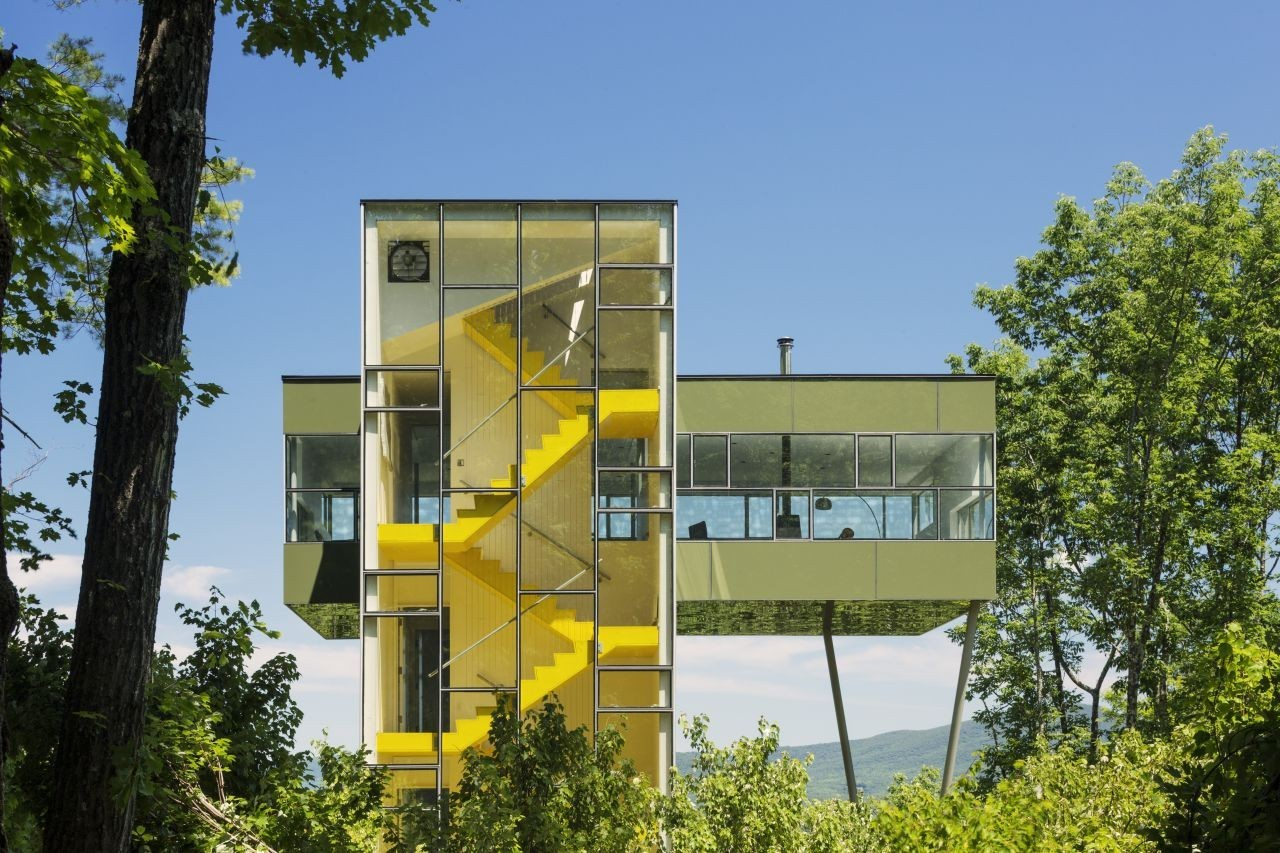
\includegraphics[width=0.9\linewidth, height=6cm]{fig1.jpg} 
\caption{}
\label{fig:subim3}
 
\end{subfigure}
\begin{subfigure}{0.5\textwidth}
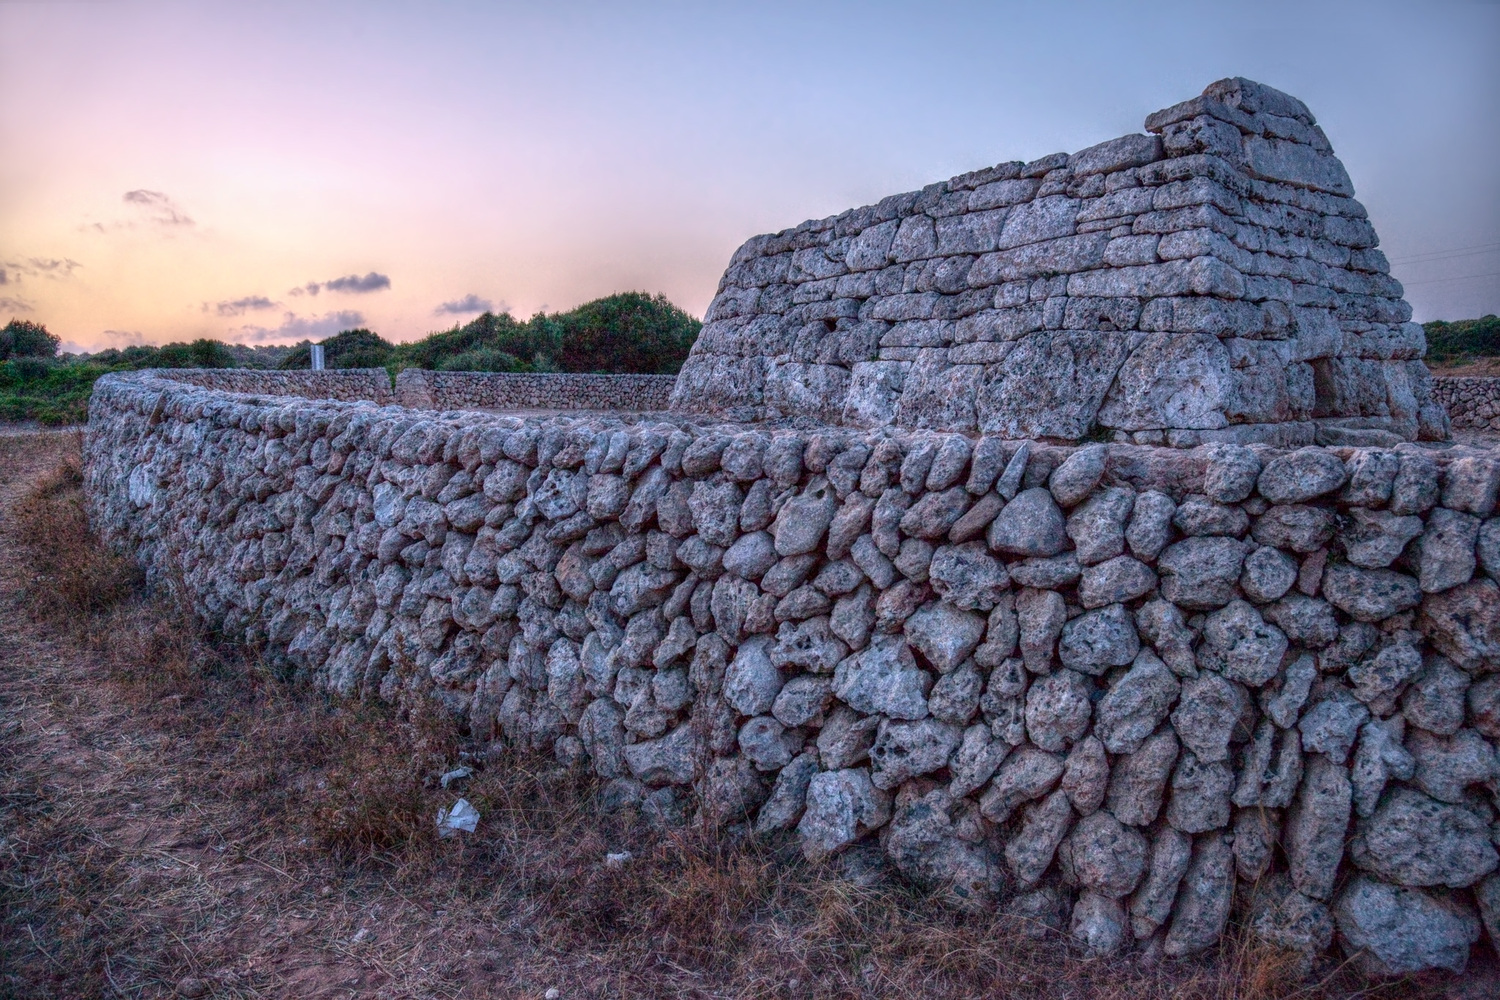
\includegraphics[width=0.9\linewidth, height=6cm]{fig2.jpg}
\caption{}
\label{fig:subim4}
\end{subfigure}
\label{fig:image3}
Images of different types of design and structure.
\end{figure}
\end{frame}

% \begin{frame}{}
% \adjustbox{right}{\insertframenumber}
\begin{figure}[h]
\begin{columns}
    \column{\dimexpr\paperwidth-10pt} 
  \end{columns}
\begin{subfigure}{0.45\textwidth}
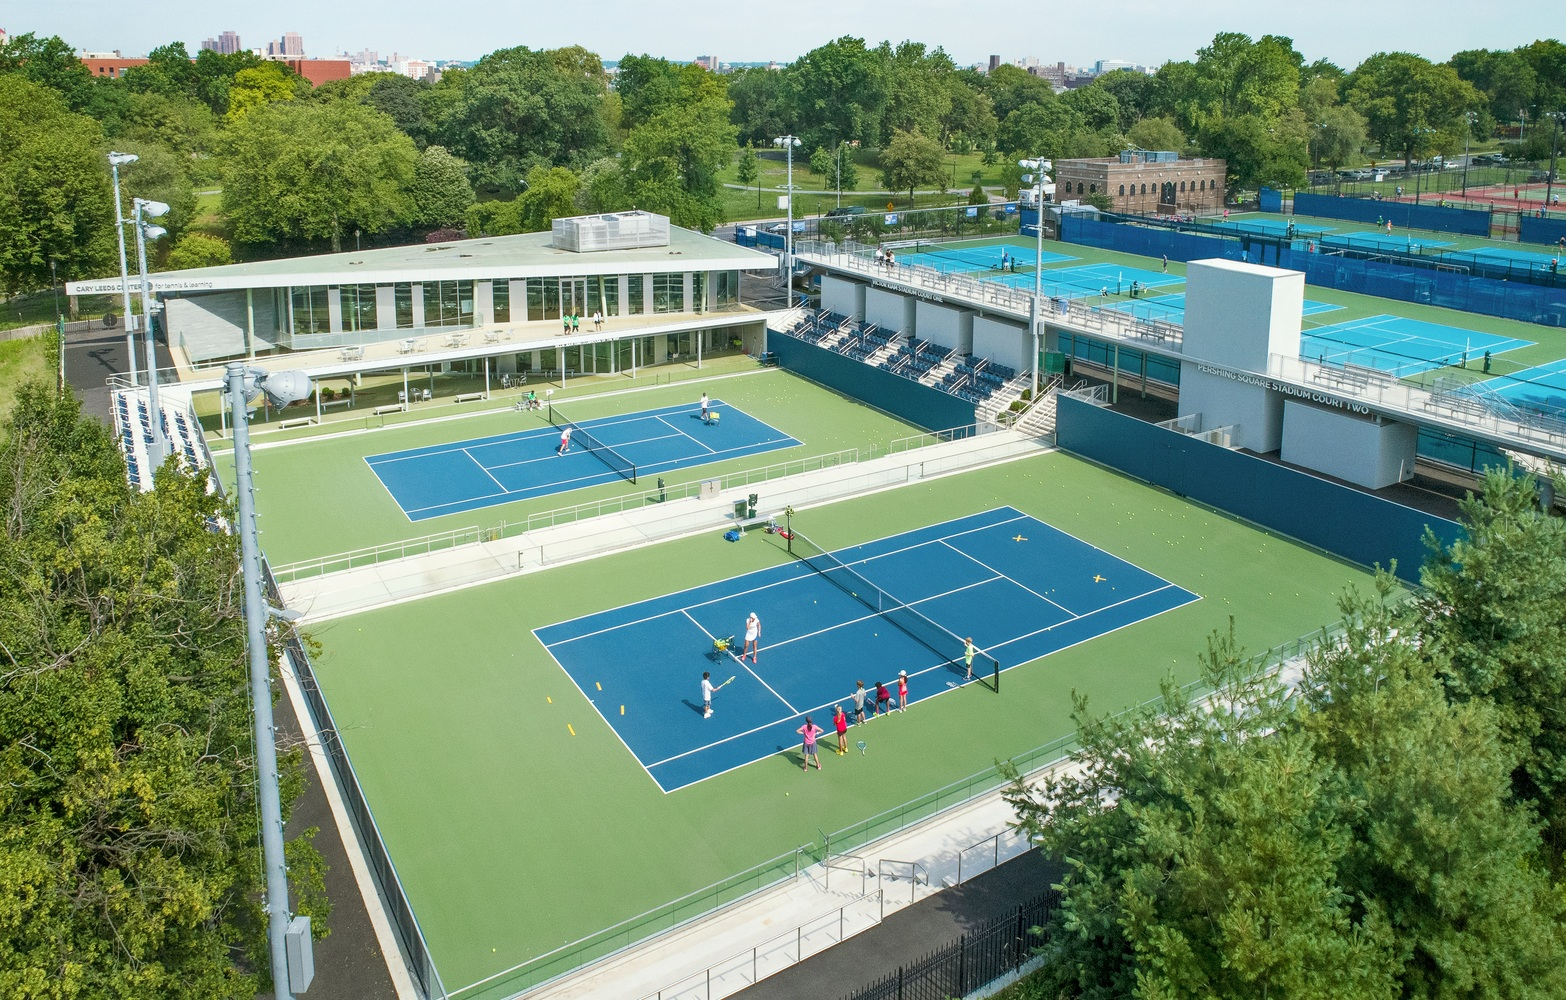
\includegraphics[width=0.9\linewidth, height=6cm]{fig3.jpg} 
\caption{}
\label{fig:subim5}
 
\end{subfigure}
\begin{subfigure}{0.5\textwidth}
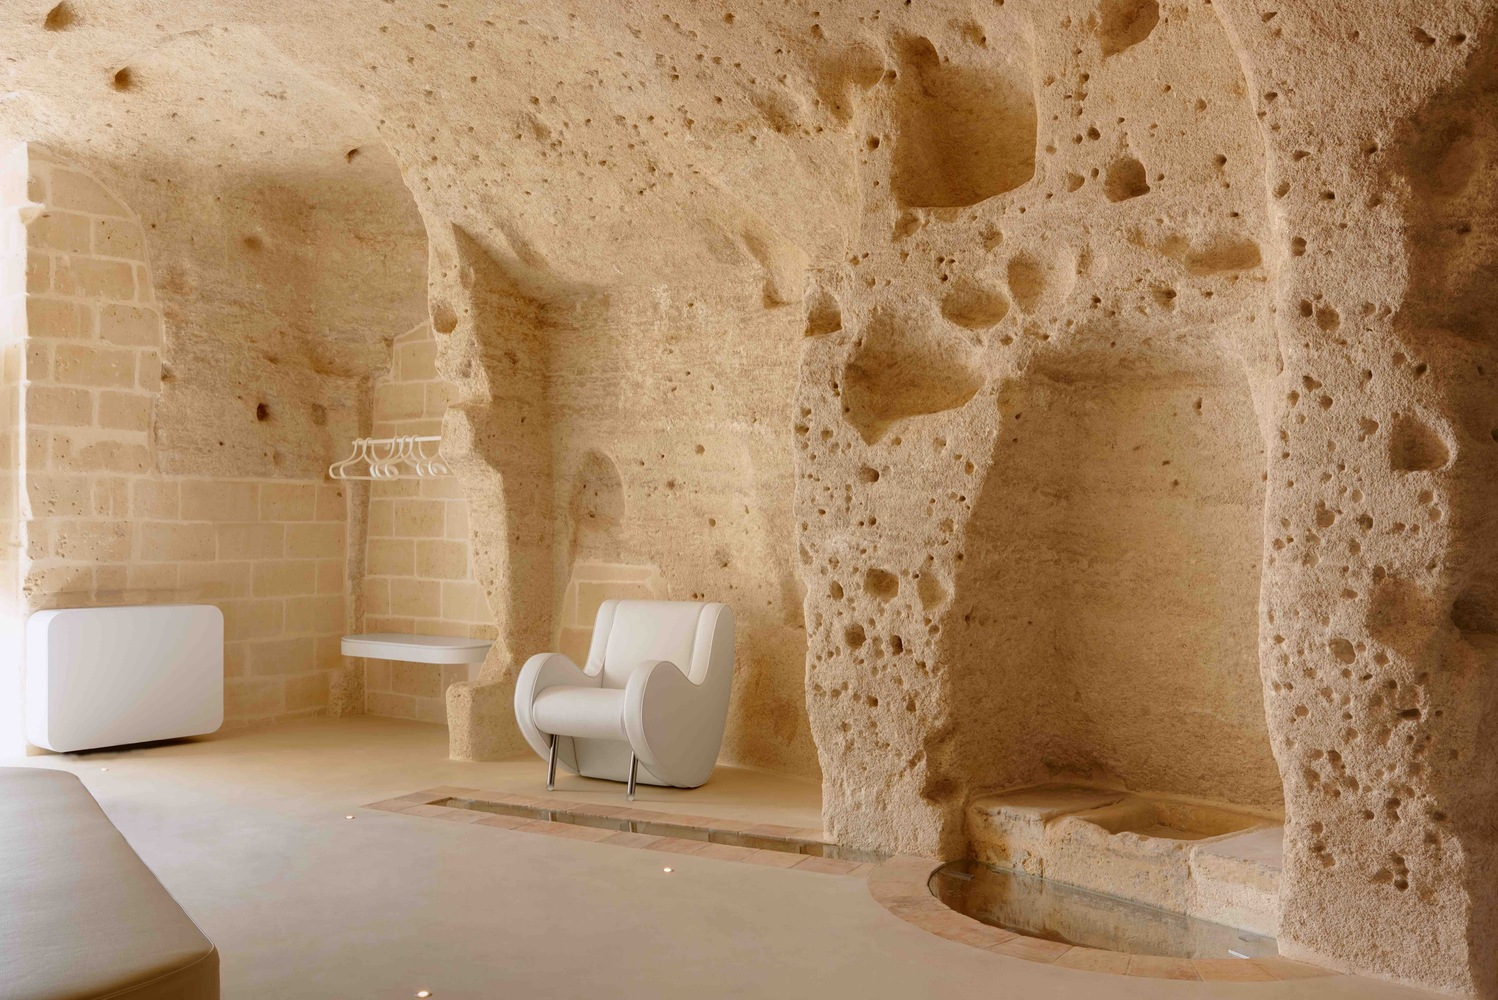
\includegraphics[width=0.9\linewidth, height=6cm]{fig4.jpg}
\caption{}
%\label{fig:subim6}
\end{subfigure}
 \label{fig:image4}
Images of uses of lightweight concrete.
\end{figure}

% \end{frame}
   
    \begin{frame}{}
        % \adjustbox{right}{\insertframenumber} 
      \begin{tikzpicture}[grow cyclic, text width=2.7cm, align=flush center,
	level 1/.style={level distance=4cm,sibling angle=30},
	]\begin{itemize} 
   \item<1->{\node{\textbf{Reduced structural load}}
       child { node {High-rise Building}}
       child { node {Long-span bridge}}
	child { node {Elevated structure}};}
    \item<2->{\adjustbox{right=7cm}{\node{\textbf{Thermal insulation}}
	child { node {Building walls}}
    	child { node {Roofs}};}}
     \end{itemize}
  \end{tikzpicture}
   \end{frame}

  \begin{frame}{}
        % \adjustbox{right}{\insertframenumber} 
      \begin{tikzpicture}[grow cyclic, text width=2.7cm, align=flush center,
	level 1/.style={level distance=4cm,sibling angle=30},
	] \begin{itemize} 
\item<1->{\node{\textbf{Reduced shrinkage and cracking}}
	child { node {Temperature 
fluctuations}}
	child { node {Humidity variations}};}
  \item<2->{\adjustbox{right=7cm}{\node{\textbf{Architectural
Flexibility}}
	child { node {Decorative
elements and
creative
designs}};}}
 \end{itemize}
  \end{tikzpicture}
   \end{frame}
   
  %  \section{\textbf{\textcolor{purple}{What is Light Weight Concrete}}}
    
  %   \begin{frame}[plain]
  %   % \adjustbox{right}{\insertframenumber}
  %       \vfill
        
  %     \centering
  %     \begin{beamercolorbox}
  %     [sep=8pt,center,shadow=true,rounded=true]{title}
  %       \usebeamerfont{title}\insertsectionhead\par%
  %       \color{oxfordblue}\noindent\rule{10cm}{1pt}
  %     \end{beamercolorbox}
  %     \vfill
  % \end{frame}
  \begin{frame}{\textbf{What is Light Weight Concrete}}
      \begin{itemize}
          \large\item[$\bullet$] <1->Lighter than conventional concrete.
           \vspace{0.5cm}
          \large\item[$\bullet$]<2->Formulated --- replacing conventional aggregate materials.
           \vspace{0.5cm}
          \large\item[$\bullet$] <3->Derived from natural or artificial materials that have inherently lower densities.
         \vspace{0.5cm}
         \item[$\bullet$]<4->Density --- 300kg/m3 to 1850kg/m3 \\ Normal concrete --- 2200kg/m3 to 2600kg/m3.
          \end{itemize}
  \end{frame}
\begin{frame}{}
\adjustbox{right}{\insertframenumber}
\begin{figure}[h]
\begin{columns}
    \column{\dimexpr\paperwidth-10pt} 
  \end{columns}
\begin{subfigure}{0.45\textwidth}
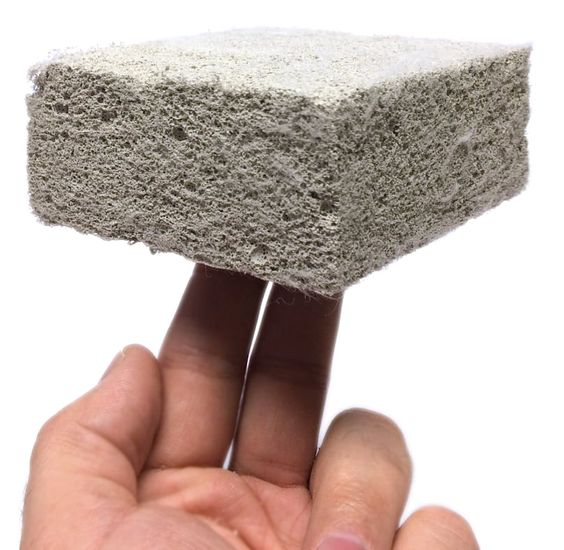
\includegraphics[width=0.9\linewidth, height=5cm]{concrete.jpg} 
\caption{}
\label{fig:subim1}
 
\end{subfigure}
\begin{subfigure}{0.5\textwidth}
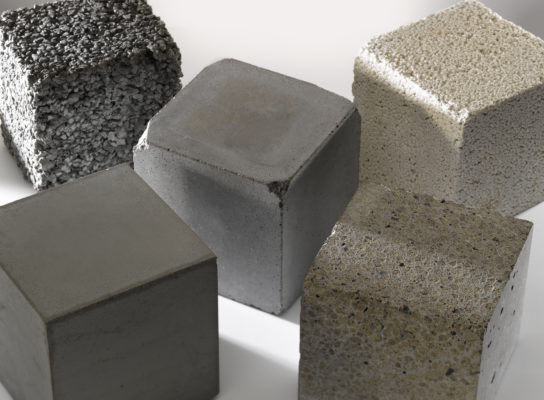
\includegraphics[width=0.9\linewidth, height=5cm]{lightweight-concrete.jpg}
\caption{}
\label{fig:subim2}
\end{subfigure}

\caption{Lightweight concrete image}
\label{fig:image2}

\end{figure}
\end{frame}
  
\begin{frame}{\textbf{Types of lightweight concrete}}
    \begin{itemize}
  \large\item[$\bullet$]<1->Three type of \textbf{{Lightweight concrete (LWC).}}.
 \item[$\empty$]<2->\begin{enumerate}
              \item Lightweight aggregate concrete.
          \end{enumerate}
          \item[$\empty$]<3->\begin{enumerate}
           \item[2.] Aerated concrete.
           \end{enumerate}
           \item[$\empty$]<4->\begin{enumerate}
           \item[3.] No-fines concrete.
               \end{enumerate}
               \vspace{0.5cm}
               \end{itemize}
  \end{frame}
 % \section{\textbf{\textcolor{purple}{Principal of LWC}}}
 %    \begin{frame}[plain]
 %     % \adjustbox{right}{\insertframenumber}
 %        \vfill
 %      \centering
 %      \begin{beamercolorbox}[sep=8pt,center,shadow=true,rounded=true]{title}
 %        \usebeamerfont{title}\insertsectionhead\par%
 %        \color{oxfordblue}\noindent\rule{10cm}{1pt}
 %      \end{beamercolorbox}
 %      \vfill
 %  \end{frame}
  \begin{frame}{\textbf{Principle Behind LWC}}
      \begin{itemize}
          \large\item[$\bullet$] <1->The basic principle behind the making of lightweight concrete is to include the air in concrete.
           \vspace{0.4cm}
          \large\item[$\bullet$]<2->To achieve the above principle practically, there are 3 different ways.
           \vspace{0.4cm}
          \large\item[$\bullet$] <3->By replacing the conventional aggregates with cellular porous aggregates
(Lightweight aggregate concrete).
         \vspace{0.4cm}
         \item[$\bullet$]<4->By incorporating the air or gas bubbles in concrete (Aerated concrete).
         \vspace{0.4cm}
         \item[$\bullet$]<5-> By omitting the sand fraction from the aggregate (No-fines concrete).
          \end{itemize}
  \end{frame}

 % \section{\textbf{\textcolor{purple}{Advantages}}}
 %    \begin{frame}[plain]
 %     % \adjustbox{right}{\insertframenumber}
 %        \vfill
 %      \centering
 %      \begin{beamercolorbox}[sep=8pt,center,shadow=true,rounded=true]{title}
 %        \usebeamerfont{title}\insertsectionhead\par%
 %        \color{oxfordblue}\noindent\rule{10cm}{1pt}
 %      \end{beamercolorbox}
 %      \vfill
 %  \end{frame}
\begin{frame}{\textbf{Advantages }}
      \begin{itemize}
          \large\item[$\bullet$] <1->Reduces the dead load of the building.
           \vspace{0.4cm}
          \large\item[$\bullet$]<2->Easy to handle and hence reduce the cost of transportation and handling.
           \vspace{0.4cm}
          \large\item[$\bullet$] <3->Improves the workability,and improved seismic performance.
         \vspace{0.4cm}
         \item[$\bullet$]<4->Relatively low thermal conductivity.
         \vspace{0.4cm}
         \item[$\bullet$]<5->Good resistance to freezing and thawing action when compared to conventional concrete.
         \vspace{0.4cm}
         \item[$\bullet$]<6->Better insulating properties and 
        superior fire resistance.
          \end{itemize}
  \end{frame}

% \section{\textbf{\textcolor{purple}{Disadvantages }}}
%     \begin{frame}[plain]
%      % \adjustbox{right}{\insertframenumber}
%         \vfill
%       \centering
%       \begin{beamercolorbox}[sep=8pt,center,shadow=true,rounded=true]{title}
%         \usebeamerfont{title}\insertsectionhead\par%
%         \color{oxfordblue}\noindent\rule{10cm}{1pt}
%       \end{beamercolorbox}
%       \vfill
%   \end{frame}
  \begin{frame}{\textbf{Disadvantages }}
      \begin{itemize}
          \large\item[$\bullet$] <1->Very sensitive to water content in the mixture.
           \vspace{0.5cm}
          \large\item[$\bullet$]<2->Volume per unit mass is more.
           \vspace{0.5cm}
          \large\item[$\bullet$] <3-> Mixing time is longer than conventional concrete to ensure proper
mixing.
         \vspace{0.5cm}
         \item[$\bullet$]<4->Lightweight concrete is porous and shows poor resistance.
         \vspace{0.5cm}
         \item[$\bullet$]<5->Slower drying time \cite{sherin2018review}.
          \end{itemize}
  \end{frame}

% \section{\textbf{\textcolor{purple}{Applications}}}
%     \begin{frame}[plain]
%      % \adjustbox{right}{\insertframenumber}
%         \vfill
%       \centering
%       \begin{beamercolorbox}[sep=8pt,center,shadow=true,rounded=true]{title}
%         \usebeamerfont{title}\insertsectionhead\par%
%         \color{oxfordblue}\noindent\rule{10cm}{1pt}
%       \end{beamercolorbox}
%       \vfill
%   \end{frame}
\begin{frame}{\textbf{Applications }}
      \begin{itemize}
          \large\item[$\bullet$] <1->It is used in the construction of roof slabs, houses with load-bearing walls, etc.
           \vspace{0.5cm}
          \large\item[$\bullet$]<2-> It is also used in the construction of stairs, windows, garden walls, etc.
           \vspace{0.5cm}
          \large\item[$\bullet$] <3->In large buildings also, this is used in the construction of partition walls.
         \vspace{0.5cm}
         \item[$\bullet$]<4->These are molded in the form of slabs and used as thermal insulators
inside the building
  \cite{mohammed2014materials}.
          \end{itemize}
  \end{frame}
% \section{\textbf{\textcolor{purple}{Properties of LWC}}}
%     \begin{frame}[plain]
%      % \adjustbox{right}{\insertframenumber}
%         \vfill
%       \centering
%       \begin{beamercolorbox}[sep=8pt,center,shadow=true,rounded=true]{title}
%         \usebeamerfont{title}\insertsectionhead\par%
%         \color{oxfordblue}\noindent\rule{10cm}{1pt}
%       \end{beamercolorbox}
%       \vfill
%   \end{frame}

%   \section{\textbf{\textcolor{purple}{Methodology
% }}}
%     \begin{frame}[plain]
%      % \adjustbox{right}{\insertframenumber}
%         \vfill
%       \centering
%       \begin{beamercolorbox}[sep=8pt,center,shadow=true,rounded=true]{title}
%         \usebeamerfont{title}\insertsectionhead\par%
%         \color{oxfordblue}\noindent\rule{10cm}{1pt}
%       \end{beamercolorbox}
%       \vfill
%   \end{frame}
% \section{\textbf{\textcolor{purple}{Case Study}}}
%     \begin{frame}[plain]
%      % \adjustbox{right}{\insertframenumber}
%         \vfill
%       \centering
%       \begin{beamercolorbox}[sep=8pt,center,shadow=true,rounded=true]{title}
%         \usebeamerfont{title}\insertsectionhead\par%
%         \color{oxfordblue}\noindent\rule{10cm}{1pt}
%       \end{beamercolorbox}
%       \vfill
%   \end{frame}
% \section{\textbf{\textcolor{purple}{Calculation}}}
%     \begin{frame}[plain]
%      % \adjustbox{right}{\insertframenumber}
%         \vfill
%       \centering
%       \begin{beamercolorbox}[sep=8pt,center,shadow=true,rounded=true]{title}
%         \usebeamerfont{title}\insertsectionhead\par%
%         \color{oxfordblue}\noindent\rule{10cm}{1pt}
%       \end{beamercolorbox}
%       \vfill
%   \end{frame}
% \section{\textbf{\textcolor{purple}{Summary}}}
%     \begin{frame}[plain]
%      % \adjustbox{right}{\insertframenumber}
%         \vfill
%       \centering
%       \begin{beamercolorbox}[sep=8pt,center,shadow=true,rounded=true]{title}
%         \usebeamerfont{title}\insertsectionhead\par%
%         \color{oxfordblue}\noindent\rule{10cm}{1pt}
%       \end{beamercolorbox}
%       \vfill
%   \end{frame}
% \section{\textbf{\textcolor{purple}{Reference}}}
%     \begin{frame}[plain]
%      % \adjustbox{right}{\insertframenumber}
%         \vfill
%       \centering
%       \begin{beamercolorbox}[sep=8pt,center,shadow=true,rounded=true]{title}
%         \usebeamerfont{title}\insertsectionhead\par%
%         \color{oxfordblue}\noindent\rule{10cm}{1pt}
%       \end{beamercolorbox}
%       \vfill
%   \end{frame}
\begin{frame}{\textbf{Methodology}}
      \begin{itemize}
          \large\item[$\bullet$] <1->Batching
           \vspace{0.4cm}
          \large\item[$\bullet$]<2->Weight batching
           \vspace{0.4cm}
          \large\item[$\bullet$] <3->Measurement of water
         \vspace{0.4cm}
         \item[$\bullet$]<4->Preparation of concrete cubes
         \vspace{0.4cm}
         \item[$\bullet$]<5->Compacting
         \vspace{0.4cm}
         \item[$\bullet$]<6->Curing
         \vspace{0.4cm}
         \item[$\bullet$]<7->Testing
          \end{itemize}
  \end{frame}
  \begin{frame}{\textbf{Conclusion and Future Scope}}
      \begin{itemize}
          \large\item[$\bullet$] <1->It is an eco-friendly alternative that can help reduce carbon emissions and promote sustainable development.
           \vspace{0.4cm}
          \large\item[$\bullet$]<2->It has a lower thermal conductivity, which makes it an excellent insulator.Higher fire resistance and sound absorption capacity
           \vspace{0.4cm}
          \large\item[$\bullet$] <3->Use of ultra-high-performance concrete panels made from lightweight
aggregates have been showcased in several projects.
         \vspace{0.4cm}
         \item[$\bullet$]<4-> More durable requires less maintenance than normal concrete.
         \vspace{0.4cm}
         \item[$\bullet$]<5->More sustainable and efficient.
For example, the use of fly ash, and paper sludge\cite{su132413893}.
          \end{itemize}
  \end{frame}
  \begin{frame}{\textbf{Conclusion and Future Scope}}
      \begin{itemize}
          \item [$\bullet$] <1-> Limitations- including lower compressive strength and potential durability concerns in certain environments.
      \end{itemize}
  \end{frame}
  
  \begin{frame}{\textbf{References}}
  
  \bibliographystyle{plain}
\thispagestyle{empty}
\bibliography{Refences.bib}

\thispagestyle{empty}

  \end{frame}
\begin{frame}{}
\thispagestyle{empty}
    \begin{center}
        \textbf{\textcolor{teal!80}{\huge  Thank You!}}
    \end{center}
\end{frame}

\end{document}


